
%% bare_conf_compsoc.tex
%% V1.4b
%% 2015/08/26
%% by Michael Shell
%% See:
%% http://www.michaelshell.org/
%% for current contact information.
%%
%% This is a skeleton file demonstrating the use of IEEEtran.cls
%% (requires IEEEtran.cls version 1.8b or later) with an IEEE Computer
%% Society conference paper.
%%
%% Support sites:
%% http://www.michaelshell.org/tex/ieeetran/
%% http://www.ctan.org/pkg/ieeetran
%% and
%% http://www.ieee.org/

%%*************************************************************************
%% Legal Notice:
%% This code is offered as-is without any warranty either expressed or
%% implied; without even the implied warranty of MERCHANTABILITY or
%% FITNESS FOR A PARTICULAR PURPOSE! 
%% User assumes all risk.
%% In no event shall the IEEE or any contributor to this code be liable for
%% any damages or losses, including, but not limited to, incidental,
%% consequential, or any other damages, resulting from the use or misuse
%% of any information contained here.
%%
%% All comments are the opinions of their respective authors and are not
%% necessarily endorsed by the IEEE.
%%
%% This work is distributed under the LaTeX Project Public License (LPPL)
%% ( http://www.latex-project.org/ ) version 1.3, and may be freely used,
%% distributed and modified. A copy of the LPPL, version 1.3, is included
%% in the base LaTeX documentation of all distributions of LaTeX released
%% 2003/12/01 or later.
%% Retain all contribution notices and credits.
%% ** Modified files should be clearly indicated as such, including  **
%% ** renaming them and changing author support contact information. **
%%*************************************************************************


\documentclass[conference,compsoc]{IEEEtran}

% *** CITATION PACKAGES ***
\usepackage[nocompress]{cite}

% *** GRAPHICS RELATED PACKAGES ***
%
\usepackage[pdftex]{graphicx}
% declare the path(s) where your graphic files are
\graphicspath{{../images/}}
% and their extensions so you won't have to specify these with
% every instance of \includegraphics
\DeclareGraphicsExtensions{.jpeg,.png}

% *** MATH PACKAGES ***
\usepackage{amsmath}
% Note that the amsmath package sets \interdisplaylinepenalty to 10000
% thus preventing page breaks from occurring within multiline equations. Use:
%\interdisplaylinepenalty=2500

% *** ALIGNMENT PACKAGES ***
\usepackage{array}

% *** SUBFIGURE PACKAGES ***
\usepackage[caption=false,font=footnotesize,labelfont=sf,textfont=sf]{subfig}

% *** FLOAT PACKAGES ***
%\usepackage{fixltx2e}
%\usepackage{stfloats}
% \usepackage{dblfloatfix}

% *** PDF, URL AND HYPERLINK PACKAGES ***
\usepackage{url}
\usepackage{bm}
%\usepackage{algorithm}
%\usepackage{algorithmic}

% *** Temporary packages ***
\usepackage{lipsum}
%\usepackage{xcolor}
%\newcommand\mytodo[1]{\textcolor{red}{#1}}

% correct bad hyphenation here
\hyphenation{op-tical net-works semi-conduc-tor}

\begin{document}

% paper title
\title{Automatic Open Domain Information Extraction\\from Indonesian Text}


% author names and affiliations
% use a multiple column layout for up to three different
% affiliations
\author{
	\IEEEauthorblockN{Yohanes Gultom}
	\IEEEauthorblockA{Faculty of Computer Science\\
	University of Indonesia\\
	Email: yohanes.gultom@ui.ac.id}
	\and
	\IEEEauthorblockN{Wahyu Catur Wibowo}
	\IEEEauthorblockA{Faculty of Computer Science\\
	University of Indonesia\\
	Email: wibowo@cs.ui.ac.id}
}


% make the title area
\maketitle

% As a general rule, do not put math, special symbols or citations
% in the abstract
\begin{abstract}

Availability of big amount digital documents calls for an automatic method to extract information from any text document regardless of domain. Unfortunately, existing open domain information extraction (open IE) methods are not suitable for low-resource language such as Indonesian. This paper introduces a method to extract relation triples from Indonesian text using a model composed of rule-based triple candidates generator, rule-based token expander and machine-learning-based triple selector. Trained using our 2,344 triples dataset (166 positives \& 2,183 negatives), a Random Forest triple selector model achieves cross-validation score of 0.58 F1 (0.62 precision and 0.58 recall).

\end{abstract}


\section{Introduction}

Open domain information extraction (open IE) is a paradigm that facilitates domain-independent discovery of triple relations from text document\cite{banko2007open}. Unlike conventional information extraction, open IE retrieves relations regardless of domain in a consistent triples format. While it uses similar format to knowledge extraction, open IE doesn't limit the extracted relation triples by certain closed ontology or relation schema\cite{auer2007dbpedia}. Relation triples produced by open IE has been reported to be useful for tasks such as question answering\cite{fader2011identifying} and information retrieval\cite{etzioni2011search}. 

The objective of open IE is to extract relation triples from a sentence

%TODO
%\item What is the research background? amount of digital documents have surpassed human ability to read, interest in machine reading (automatic, unsupervised, understanding of text), traditional ie is limited, knowledge extraction uses NLP tasks which requires datasets that are not available for low-resource language such as Indonesian, openie definition, openie relies on language specific heuristics
%\item What is the research problem? develop baseline model and implementation for Indonesian openie
%\item How does this research address the problem? Proposes a model that combine heuristics (rule-based) and supervised learning models for Indonesian language, provides dataset and opensource implementation
%\item What is the contribution of this paper? model of open IE for Indonesian text, implementation of the model, manually tagged dataset of triple selection, reusable NLP pipeline to annotate lemma, part of speech, named-entity and dependency of Indonesian text
%\item How is this paper organized? Introduction, related works, model details, experiments, analysis, conclusion and future works
%\end{itemize}



\lipsum[1-2]

\begin{figure}
\textbf{Input} \\[0.1cm]
"Sembungan adalah sebuah desa yang terletak di kecamatan Kejajar, kabupaten Wonosobo, Jawa Tengah, Indonesia." \\[0.5cm]
\textbf{Output} \\[0.1cm]
1. (Sembungan, adalah, desa) \\
2. (Sembungan, terletak di, kecamatan Kejajar) \\
\caption{Example of expected input and output of open domain information extraction}
\label{fig_example_io_openie}
\end{figure}

\section{Related Works}

TextRunner was designed for massive size of open-domain web documents by avoiding heavy linguistic tasks and used inverted index to store extraction result\cite{banko2007open}. It generates its own dataset (self-supervised) by using part of speech and dependency features and train a naive bayes classifier to select the triples. It argues that heavy linguistic tasks such as dependency parsing are not scalable to handle million of web documents. Additionally, it also uses redundancy assessor to remove redundant words (stop words, adverbs .etc).

ReVerb is an immediate successor of TextRunner which solves two significant problems in its predecessor: incoherent extractions and uninformative extractions \cite{fader2011identifying}. It is composed of two algorithm: (1) Relation Extraction that extracts relations using syntactical and lexical constraint to solve the problems, and (2) Argument Extraction which retrieve the noun phrases as arguments of the relation. ReVerb takes as input a POS-tagged and NP-chunked and returns a set of relation triples.

R2A2 is a system built to fix argument extraction problem in ReVerb \cite{etzioni2011open}. Instead of using heuristics to extract the arguments, it uses a learning-based system, ArgLearner, that accepts relation and sentence as inputs and returns the first (Arg1) and second arguments (Arg2). ArgLearner extracts the arguments using three classifiers based on REPTree and sequence labeling CRF as described in Figure \ref{fig_arglearner_architecture}.

\begin{figure}
\centering
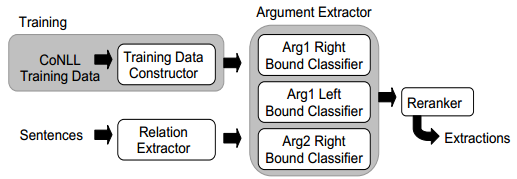
\includegraphics[scale=0.3]{arglearner_architecture}
\caption{ArgLearner architecture training and extraction architecture}
\label{fig_arglearner_architecture}
\end{figure}

Furthermore, Ollie (Open Language Learning for Information Extraction) utilizes ReVerb to learn open pattern templates to guide triples extraction from sentence. Additionally, Ollie does a context analysis to extend the tuples with contextual information in order to improve precision. Its training and extraction architecture is describe in Figure \ref{fig_ollie_architecture}.

\begin{figure}
\centering
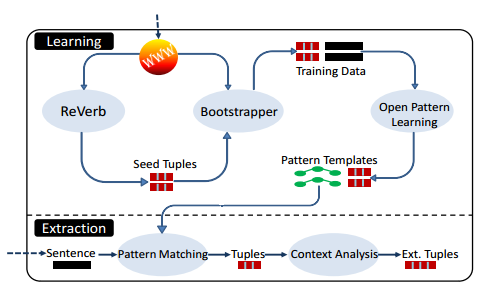
\includegraphics[scale=0.3]{ollie_architecture}
\caption{Ollie training and extraction architecture}
\label{fig_ollie_architecture}
\end{figure}

\section{Proposed Models}

\begin{figure*}[!t]
\centering
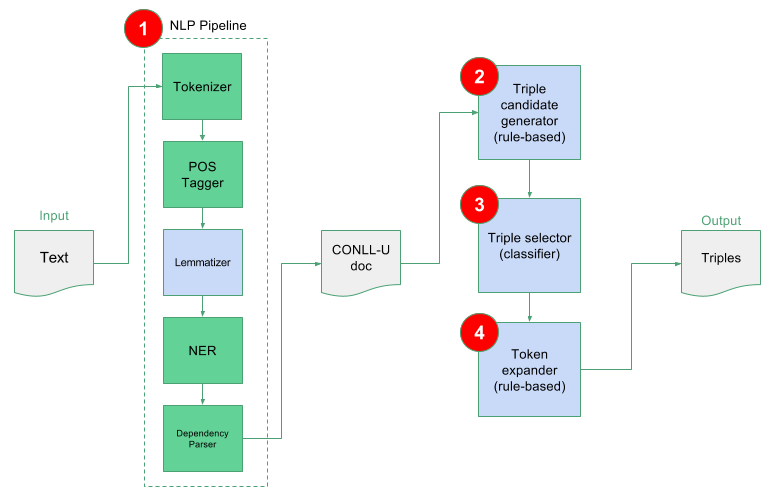
\includegraphics[width=\textwidth]{program_flowchart}
\caption{Program flowchart}
\label{fig_program_flowchart}
\end{figure*}

%Generally is similar to TextRunner
%
%TextRunner, automatically tag the triples candidates\cite{banko2007open} while we combine automatic candidates generator with manual (human) annotation
%
%These model is based on three-step method of Label, Learn, Extract\cite{etzioni2011open} but use the mix of heuristics and manual labeling

\lipsum[1]

\subsection{NLP Pipeline}

\lipsum[3-5]

\begin{figure}
\centering
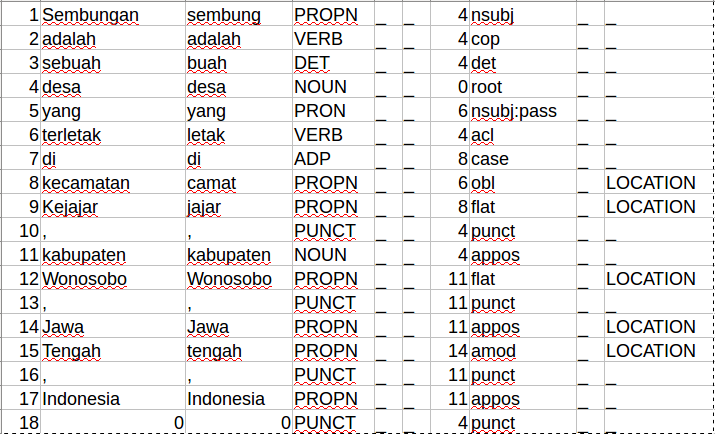
\includegraphics[scale=0.35]{conllu_example}
\caption{CONLL-U Format Example}
\label{fig_conllu_example}
\end{figure}

\subsection{Triple Candidate Generator}

% Similar to TextRunner Self-Supervised Learner but doesn't automatically label triples

\lipsum[3-5]

% Triple candidate generation rules
\begin{table}[!t]
\renewcommand{\arraystretch}{1.5}
\caption{Triple candidate generation rules}
\label{table_triple_candidate_generation_rules}
\centering
\begin{tabular}{l|p{6cm}}
\hline
\textbf{Type} & \textbf{Condition} \\
\hline
Subject & Token's POS tag is either PROPN, NOUN, PRON or VERB \\
\space & Token is not "yang" nor "adalah" \\
\space & Token's dependency is neither "compound" nor "name" \\
\space & Token's dependency is either "compound" or "name" but separated by more than 2 tokens from its head \\
\hline
Predicate & Token's position is after Subject \\
\space & Token's POS tag is either VERB or AUX \\
\hline
Object & Token's position is after Subject and Predicate \\
\space & Token's POS tag is either PROPN, NOUN, PRON or VERB \\
\space & Token is not "yang" nor "adalah" \\
\space & Token's dependency is neither "compound" nor "name" \\
\space & Token's dependency is either "compound" or "name" but separated by more than 2 tokens from its head \\
\end{tabular}
\end{table}


\subsection{Triple Selector}

%Similar to TextRunner Self-Supervised Learner but uses dependency-based and NER-based features
%While TextRunner uses Naive Bayes Classifier, our model uses other models such as Logistic Regression, SVM, MLP and Random Forest

\lipsum[3-5]

\begin{table}[!t]
\renewcommand{\arraystretch}{1.5}
\caption{Triple selector features}
\label{table_models_features}
\centering
\begin{tabular}{r|l}
\hline
\textbf{\#} & \textbf{Features} \\
\hline
1 & Subject token's POS tag \\
2 & Subject token's dependency relation \\
3 & Subject token's head POS tag \\
4 & Subject token's named entity \\
5 & Subject token's distance from predicate \\
7 & Subject token's dependency with predicate \\
8 & Predicate token's POS tag \\
9 & Predicate token's dependency relation \\
10 & Predicate token's head POS tag \\
11 & Predicate token's dependents count \\
12 & Object token's POS tag \\
13 & Object token's dependency relation \\
14 & Object token's head POS tag \\
15 & Object token's named entity \\
16 & Object token's dependents count \\
17 & Object token's distance from predicate \\
18 & Object token's dependency with predicate \\
\end{tabular}
\end{table}


\subsection{Token Expander}

%While TextRunner uses lightweight noun phrase chunker, our models uses rule-based token expander to find entities (subject or object token) 

\lipsum[3-5]

% Token expansion rules for Subject or Object token
\begin{table}[!t]
\renewcommand{\arraystretch}{1.5}
\caption{Token expansion rules for Subject or Object token}
\label{table_token_expansion_rules_s_o}
\centering
\begin{tabular}{r|p{6cm}|l}
\hline
\textbf{\#} & \textbf{Condition for Subject or Object Token} & \textbf{Action} \\
\hline
1 & If dependent's relation to the token  is either “compound”, “name”  or “amod” & Expand \\
2 & If dependent has same named entity as the token & Expand \\
3 & If dependent and the token are wrapped by quotes or double quotes  & Expand \\
4 & If the head is a sentence root & Ignore \\
5 & If dependent's POS tag is CONJ or its form is either “,” (comma) or “/” (slash) & Ignore \\
6 & If dependent's POS tag is either “VERB” or “ADP” & Ignore \\
7 & If dependent has at least one dependent with “ADP” POS tag & Ignore \\
8 & If the first or last token in expansion result has “CONJ” or “ADP” POS tag & Remove \\
9 & If the first or last index of expansion result is an incomplete parentheses symbol & Remove \\
10 & If the last index of expansion result is “yang” & Remove \\
11 & Else & Ignore \\

\end{tabular}
\end{table}

\begin{table}[!t]
\renewcommand{\arraystretch}{1.5}
\caption{Token expansion rules for Predicate token}
\label{table_token_expansion_rules_p}
\centering
\begin{tabular}{r|p{6cm}|l}
\hline
\textbf{\#} & \textbf{Condition for Predicate Token} & \textbf{Action} \\
\hline
1 & If dependent is “tidak” & Expand \\
2 & Else & Ignore \\
\end{tabular}
\end{table}

\section{Experiments}

%2 sentences document, 7 triples, 6.157 seconds (0.8 seconds per sentence)  (Core i7 5500U)
%138 sentences document, 429 triples, 11.324 seconds (0.082 seconds per sentence) (Core i7 5500U)
%5,593 sentences document, 19,403 triples, 78.623 seconds (0.014 seconds per sentence)  (Core i7 5500U)
%Our system is quite scalable (faster on bigger document)
%Our system has a comparable speed with TextRunner

\lipsum[1-2]

\begin{figure}
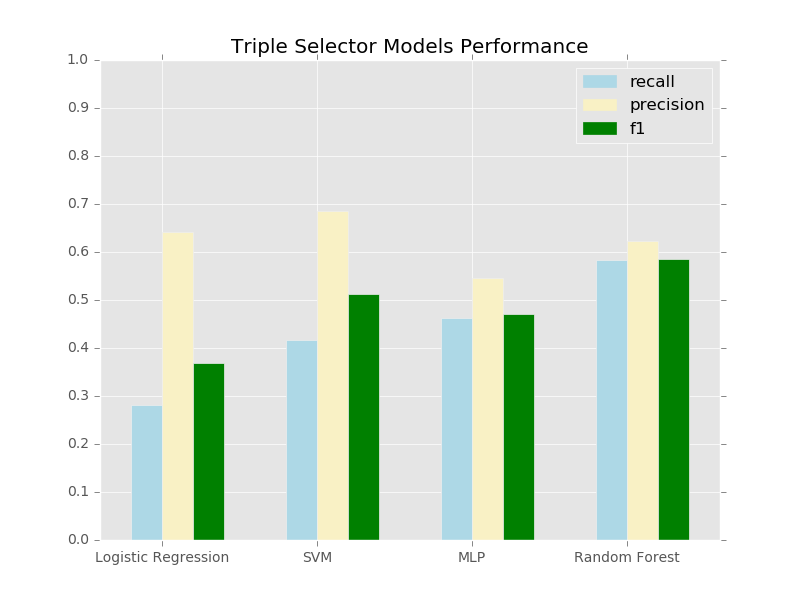
\includegraphics[scale=0.4]{models_performance}
\caption{Triple selector models performance comparison chart}
\label{fig_models_performance}
\end{figure}

\begin{table}[!t]
\renewcommand{\arraystretch}{1.5}
\caption{Triple selector models performance}
\label{table_models_performance}
\centering
\begin{tabular}{l r r r}
\hline
\textbf{Models} & \textbf{P} & \textbf{R} & $\mathbf{F_1}$ \\
\hline
Logistic Regression & 0.64 & 0.28 & 0.36 \\
SVM & \textbf{0.68} & 0.41 & 0.51 \\
MLP & 0.54 & 0.46 & 0.47 \\
Random Forest & 0.62 & \textbf{0.58} & \textbf{0.58} \\
\hline
\end{tabular}
\end{table}

\section{Analysis}

\lipsum[6-7]

\section{Conclusion}

%Introduces open ie extraction model for Indonesian text
%Provides open-source working implementation of the model

Future works
Extract implicit relations in sentence using better heuristics
Use machine learning model for token expansion
Estimate confidence level in every phases (NLP pipelines, candidate generator, triple selector, token expander) for following process
Use better feature extraction using Word2Vec and deep learning
Optimize system to handle large number of documents

\lipsum[6-7]

% conference papers do not normally have an appendix

% use section* for acknowledgment
%\ifCLASSOPTIONcompsoc
  % The Computer Society usually uses the plural form
%  \section*{Acknowledgments}
%\else
  % regular IEEE prefers the singular form
%  \section*{Acknowledgment}
%\fi

\bibliographystyle{IEEEtran}
\bibliography{../pustaka}

% that's all folks
\end{document}
